\documentclass[journal]{IEEEtran}
\usepackage{graphicx}
\begin{document}

\title{ How the observer Pattern in FreeCol affect extendability and usability as measured by NOP}

\author{Karl Fredrik Gudjonsson\\
        Link\"{o}pings University, Sweden\\
        kargu328@student.liu.se
}
\markboth{TDDB84 - Design Patterns, October 2015}
{Shell \MakeLowercase{\textit{et al.}}: Bare Demo of IEEEtran.cls for Journals}

\maketitle
\begin{abstract}
The abstract goes here. This paper research if the implementation of the Observer pattern increase the maintainability/extendability in FreeCol...
\end{abstract}

\begin{IEEEkeywords}
Design patterns; FreeCol; JAVA; NOP;\\ Observer Pattern
\end{IEEEkeywords}
\IEEEpeerreviewmaketitle
\section{Introduction}
\IEEEPARstart{O}{ne} of the hardest problems to solve in programming is to develop a good software design, in order to keep the project easy to understand, extensible, maintainable, and efficient. A solution to this  are thought to be using design patterns when designing software. The main advantages of using design patterns are\cite{zhang2012we}:
\begin{enumerate}
\item {Using design patterns improves the programmer productivity and the software quality.}
\item{Beginners can increase their programming skills by applying design patterns in their learning process, by recognizing similarities between problems they encounter.}
\item{Design patterns improves the understanding between both developers and maintainers working on the same project}
\end{enumerate}

As of yet there are no concrete evidence for this, and this subject needs further studying. However there are some claims that supports that the use of design patterns improves the understanding between developers and maintainers. This papers main focus is how the use of the observer pattern in \textit{FreeCol} improves the maintainability/extendability.
\\
\\
In this paper the aim is to answer the following question:
\\
\\
How does the implementation of observer patters in FreeCol affect the maintainability and extendability as measured by NOP (number of polymorphic methods)?

\section{Theory}
\subsection{Design Patterns}
Design patterns are a way of structuring code to solve reoccurring problems when designing software. A design pattern is not a final design that can be copied straight into the source code. It is more of a description for how to solve a problem. \cite{Usefulnessofdesign}

\subsection{The Observer Pattern}
The observer pattern goes under the category of behavioral patterns, with the intet to: "Define a one-to-many dependency between objects so that when one object changes state, all its dependents are notified and updated automatically." \cite{gof}
\begin{figure}[h]
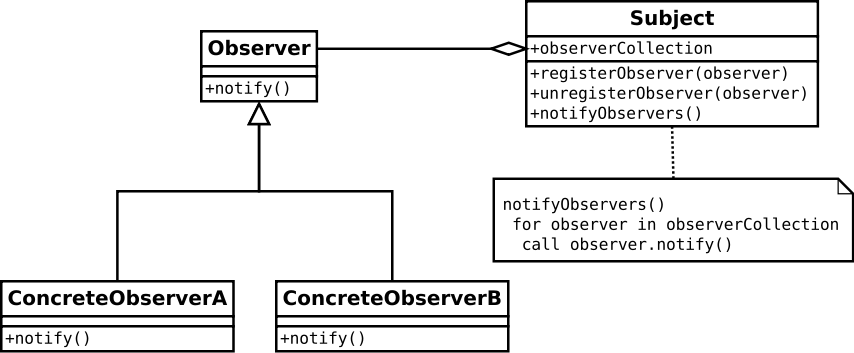
\includegraphics[width=0.5\textwidth]{Observer.png}
\label{obeserver}
\caption{UML-diagram of the Observer pattern \cite{observerpng}}
\end{figure}

The problem we want to solve by using the observer pattern is to contain consistency between objects that all depend on the same data. The observer pattern consists of one subject class containing a state which is of interest of different observer classes, and notifies the observer when there are changes made.

\subsection{FreeCol}
FreeCol is an open source game written in JAVA based on the turn-based strategy game Colonization\cite{freecol}. In this paper the focus in the code will be in and arround the class \textbf{net.sf.freecol.common.model.TrasactionListener.java}.

\section{method}
\subsection{Number of polymorphic methods}
The number of  methods that are using polymorphism (the ability to override an existing method when compiling or running the program)  to override a method of a base class. The purpose of using this is mainly to increase the extendability and flexibility. But this comes with the cost of the design being harder to understand \cite{qualityassessment}.
\section{result}
Results goes here.
\section{analysis}
Analysis goes here.
\section{Conclusion}
The conclusion goes here.
\newpage

\bibliographystyle{IEEEtran}
\bibliography{references}


\end{document}
